\section{Übersicht der Systemarchitektur}
\setauthor{Simon Koll}
\begin{figure}[h]
    \centering
    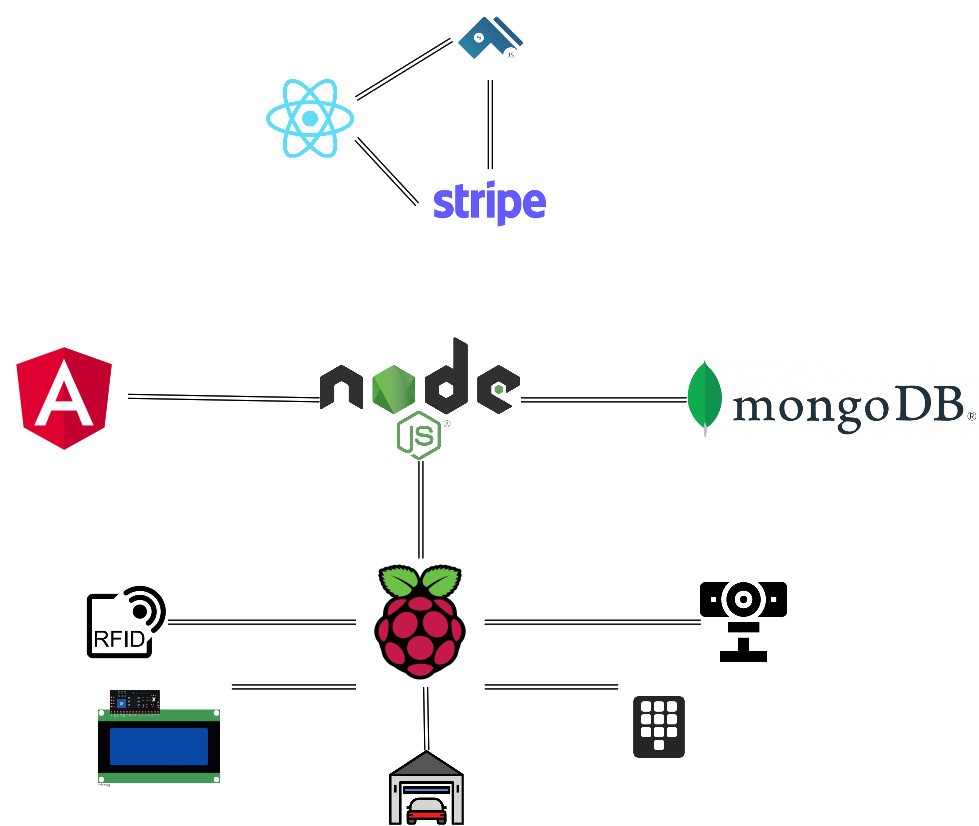
\includegraphics[width=10cm]{pics/APERTASystemarchitektur.jpg}
    \caption{Systemarchitektur}
    \end{figure}
Diese Diplomarbeit setzt sich aus zwei voneinander unabhängigen Systemen zusammen. Das Shopsystem, bestehend aus einem React-Frontend, kommuniziert mit zwei Bibliotheken, CommerceJS und Stripe, welche für die Produktverwaltung, sowie den Bezahlvorgang zuständig sind. Das Angular-Frontend des Dashboard in Verbindung mit dem NodeJS Server, der MongoDB Datenbank sowie dem Raspberry bietet das zweite System.
<<<<<<< HEAD
Der Raspberry ist über GPIOs mit dem RFID-Leser, dem Nummernfeld und dem Display verbunden. Weiters wurde die Kamera an einen der USB 3.0 Ports des Raspberry angeschlossen.
\section{Frontend (Angular-Applikation) [DH]}
=======
Der Raspberry ist über GPIOs mit dem RFID-Leser, dem Nummernfeld und dem Display verbunden. Weiters wurde die Kamera an einen der USB 3.0 Ports des Raspberry angeschlossen. Wird eine der Zutrittsmöglichkeiten positiv abgeschlossen, steuert der Raspberry Pi das Relais an, welches die Garage öffnet.
\section{Frontend (Angular-Applikation)}
>>>>>>> 8b2d001391dd8d26c7e90d13a7e95efb34cf0421
\setauthor{David Hauser}

Die Profilseite ist ein wichtiger Teil des webbasierten Clients, jedoch gibt es für die einzelnen Bauteile auch eigene Unterseiten. Auf diesen Seiten hat die Benutzerin oder der Benutzer noch mehr Möglichkeiten über die Komponenten zu entscheiden. Um die Daten für den Raspberry Pi bereitstellen zu können, werden noch weitere Funktionen benötigt.

\subsection{Aufbau von Angular}

\begin{figure}[h]
    \centering
    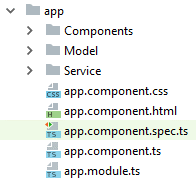
\includegraphics[width=0.4\textwidth]{pics/Aufbau_Angular.png}
    \caption{Aufbau eines Angular Projekts}
    \end{figure}

Die Applikation ist, wie bei Angular-Projekten üblich, in unterschiedliche Ordner aufgeteilt. Der App-Ordner besitzt mehrere Unterordner, welche ähnliche Funktionen gruppieren.

\subsubsection{App}
Die Dateien, welche mit app.component beginnen, werden als App bezeichnet. Sie stellen die Hauptkomponente der Angular-Applikation dar. Für das Routing im Projekt könnte noch eine app-routing.module.ts Datei angelegt werden. Wird diese nicht erstellt, kann das Routing auch in der app.module.ts durchgeführt werden.

\begin{lstlisting}[caption=app.module.ts]
    @NgModule({
  declarations: [
    AppComponent,
    ProfileComponent,
    NfcSettingsComponent,
    KeyPadSettingsComponent,
    SignSettingsComponent,
    LoginComponent,
    NavbarComponent,
    KeypadComponent,
    SignComponent
  ],
  imports: [
    BrowserModule,
    BrowserAnimationsModule,
    [RouterModule.forRoot(routes)],
    MatCardModule,
    ReactiveFormsModule,
    MatFormFieldModule,
    MatInputModule,
    MatButtonModule,
    MatSelectModule,
    MatRadioModule,
    MatIconModule,
    HttpClientModule
  ],
  providers: [],
  exports: [RouterModule],
  bootstrap: [AppComponent]
})
export class AppModule { }
\end{lstlisting}

In dieser Datei finden die Imports der Node-Module statt. Zusätzlich werden auch die verwendeten Services importiert. Die Module werden unterteilt, um sie strukturierter zu speichern. Außerdem werden die Angular Materials Module importiert, welche der Programmiererin oder dem Programmierer helfen, die Applikation leichter zu gestalten. 

\begin{lstlisting}[caption=Routing der Komponenten in der app.module.ts]
const routes: Routes = [
  { path: '', component: LoginComponent },
  { path: 'profile', component: ProfileComponent },
  { path: 'nfcSettings', component: NfcSettingsComponent},
  { path: 'keyPadSettings', component: KeyPadSettingsComponent},
  { path: 'signSettings', component: SignSettingsComponent},
  { path: 'addSign', component: AddSignComponent },
  { path: 'login', component: LoginComponent},
  { path: 'nav', component: NavbarComponent}
];
\end{lstlisting}

Mittels [RouterModule.forRoot(routes)] werden die Routen innerhalb des Projekts definiert. Sie navigieren die Userin oder der User durch die einzelnen Views.

Um den Pfad einer Route zu bestimmen wird der Pfadname angegeben.  Darauf folgt die Komponente, welche aufgerufen werden soll.

\begin{lstlisting}[caption=app.component.html]
    <app-navbar></app-navbar>
    <router-outlet></router-outlet>    
\end{lstlisting}

Diese html-Datei ist der Kern der Anwendung. Mittels <app-navbar> wird die Navbar eingebunden, welche dauerhaft am Client angezeigt wird. Im Befehl <router-outlet> werden die Komponenten, die bei den Routen im app.module.ts angegeben sind, angezeigt.

\subsubsection{Komponenten}
In diesem Ordner sind alle Komponenten auffindbar, die in der Anwendung verwendet werden. Es sind also alle Seiten mit ihren Unterkomponenten, wobei eine Seite eine gesamte Komponente darstellt, zu finden.

\subsubsection{Service}
Dieser Ordner beinhaltet alle Dienste für die Applikation. Die Funktionsweise und Verwendung wird nachfolgend noch genauer beschrieben.

\subsection{Angular-Komponente}
Die Anzeigeelemente in Angular werden als Komponenten bezeichnet. Diese werden als eigene HTML-Elemente definiert. Sie stellen abhängig von ihrer Anzeige-Logik und den Daten den Zustand der Anwendung dar.

\begin{figure}[h]
    \centering
    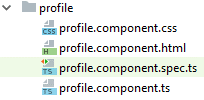
\includegraphics[width=0.4\textwidth]{pics/Aufbau_Komponente.png}
    \caption{Aufbau einer Angular Komponente}
\end{figure}

Jede Komponente besteht aus:

\begin{itemize}
    \item HTML
    \item CSS
    \item TypeScript
    \item spec.TypeScript 
\end{itemize}

Wie sich die Komponente verhält und welche Daten sie anzeigt, wird in der TypeScript Klasse definiert. Ihr Aussehen und wo die Daten genau angezeigt werden sollen, wird in der HTML-Datei festgelegt. Ihr Design kann über das CSS-File bestimmt und beeinflusst werden.
\cite{AngularKomponenten}

\subsection{Services}
Für die Daten und Logik, welche nicht nur in einer Komponente verwendet werden, werden Angular Services genutzt. Darin werden Attribute und Methoden definiert, welche anschließend von anderen Komponenten und Services verwendet werden können.

\begin{figure}[h]
    \centering
    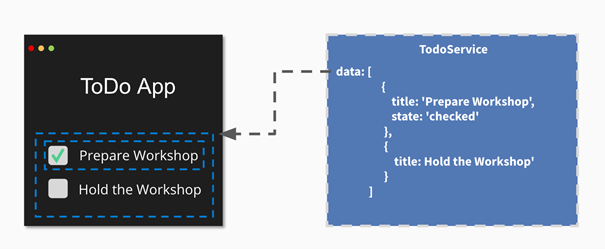
\includegraphics[width=0.8\textwidth]{pics/Service_Klasse.png}
    \caption{Auslagern einer Service Klasse}
    \cite{Service}
\end{figure}

Das Service liefert also die eigentlichen Daten für die Komponente. Die Daten gehören nicht in die Komponente. Explizite Aufgaben sollten in einem entsprechenden Service ausgelagert werden. Um die ausgelagerten Daten dann in die Komponente zu bekommen, wird Dependency Injection verwendet.

Dependency Injection
Unter Dependency Injection oder auch Inversion of Control wird ein Design-Pattern verstanden. Die Dependency sollte also nicht von der aufrufenden Stelle selbst erzeugt werden. Letztere sollte die Kontrolle abgeben und nur die Abhängigkeiten definieren. 

In Angular werden die verschiedenen Services vom sogenannten Injector verwaltet. Dieser gibt eine Referenz des Service und die aufrufende Stelle an, sofern dieser definiert ist. Über den Konstruktor wird die Definition der Abhängigkeit abgebildet. In einem Konstruktor können dann die Methoden des Service aufgerufen und somit auf die Daten zugegriffen werden.
\cite{AngularService}

\section{Frontend (React-Applikation)}
\setauthor{Benjamin Golic}
